
\documentclass[sigconf]{acmart}

%% \BibTeX command to typeset BibTeX logo in the docs
\AtBeginDocument{%
  \providecommand\BibTeX{{%
    \normalfont B\kern-0.5em{\scshape i\kern-0.25em b}\kern-0.8em\TeX}}}

%% Rights management information.  This information is sent to you
%% when you complete the rights form.  These commands have SAMPLE
%% values in them; it is your responsibility as an author to replace
%% the commands and values with those provided to you when you
%% complete the rights form.
\setcopyright{acmcopyright}
\copyrightyear{2018}
\acmYear{2018}
\acmDOI{10.1145/1122445.1122456}

%% These commands are for a PROCEEDINGS abstract or paper.
\acmConference[Woodstock '18]{Woodstock '18: ACM Symposium on Neural
  Gaze Detection}{June 03--05, 2018}{Woodstock, NY}
\acmBooktitle{Woodstock '18: ACM Symposium on Neural Gaze Detection,
  June 03--05, 2018, Woodstock, NY}
\acmPrice{15.00}
\acmISBN{978-1-4503-XXXX-X/18/06}


%% end of the preamble, start of the body of the document source.
\begin{document}

%% Title used for page headers
\title{Taxulator – The Smart Way to File Taxes}

% Authors
\author{Elisha Coad}
\affiliation{%
  \institution{Department of Computer Science}
  \institution{University of Idaho}
  \city{Moscow}
  \country{USA}}
\email{coad1223@vandals.uidaho.edu}

\author{Cade Disselkoen}
\affiliation{%
  \institution{Department of Computer Science}
  \institution{University of Idaho}
  \city{Moscow}
  \country{USA}}
\email{diss7248@vandals.uidaho.edu}

\author{Ryan Rapier}
\affiliation{%
  \institution{Department of Computer Science}
  \institution{University of Idaho}
  \city{Moscow}
  \country{USA}}
\email{rapi3147@vandals.uidaho.edu}

\author{Hasan Jamil}
\affiliation{%
  \institution{Department of Computer Science}
  \institution{University of Idaho}
  \city{Moscow}
  \country{USA}}
\email{jamil@uidaho.edu}


%% Abstract
\begin{abstract}
  For decades, taxes have remained the same. People are expected to keep meticulous record of all their income and spending over the year and then spend hours filling out a tax report. While the effort put into this is commendable, what if there’s a better way? In this paper, we describe the implementation of Taxulator, a quicker and easier way to file yearly taxes. Through collecting forms from all respective parties beforehand, the individual taxpayer is able to file taxes in a matter of minutes.
\end{abstract}

% CCS Concepts
\ccsdesc[500]{Information systems~Data management design and models}
\ccsdesc[500]{Computing methodologies~Information extraction}
\ccsdesc{Computing methodologies~PDF parsing}

% Keywords
\keywords{tax reports, query language, congregate user system, information extraction, user profile management system}

%% This command builds the first part of the formatted document.
\maketitle

\section{Introduction}
\subsection{Motivation}
In the United States of America, taxes have always been a complex system. It requires much leg work on the individual taxpayer and because of this is often dreaded. This is the motivation behind the Taxulator program, to streamline the tax filing process.
A secondary motivation though would be to bring the benefits of technology to tax filing. Such benefits include security, clarity, and easy record keeping. Security in receiving private financial information directly from the source, without the possibility of interception. Clarity in providing additional information through the tax filing process, so that fewer mistakes are made overall. And record keeping, for a digital report is much easier to find and pull up than searching for the same report in boxes of old files.
\subsection{Research}
Previous research shows there are a few tax solutions already out there. One can hire someone to do their taxes for them. This method works but is hands-off and a bit costly. There are also several tax websites, such as TurboTax and FreeTaxUSA, but very few use a centralized filing scheme. This means that most still require the individual taxpayer to upload all of their employer forms, investment interest forms, rental income forms, and more. What we propose is that these forms are submitted directly by their respective parties, helping reduce overall amount of work required.
\subsection{Challenges}
As one might expect, a collaborative tax filing process such as the one Taxulator is looking to employ, has its challenges. For one, it’s a scheme that requires the cooperation of multiple parties to work. For a single tax filing, the employers must report salaries, banks must report investment interests, rentals must be reported by the renters and the list goes on. To help speed up its adoption rate, will be deployed in controlled areas where the companies and banks in that area will be encouraged to adopt using Taxulator as part of their process. If we can get a few cities fully onboard the Taxulator system, the hope is that its usefulness will catch on and it will spread outward to other cities.
Another challenge with creating any digital system that deals with finances is security. We will be dealing with highly private information and as such will need highly secure systems. To do this, our goal is to limit our access to the customer’s info and documents as much as possible, so that only the parties who need the information will have access. We will also be utilizing extremely secure encryption methods so that in the unlikely event there is a security breach, all data will be unrecognizable.
The last challenge that will be discussed is the difficulty of collating data from multiple different sources and documents into one place. There will be multiple forms from multiple enterprises, each requiring different treatment. This challenge though can be overcome through simply brute force. We will ensure we have methods of handling each unique form. In the odd case of a form being needed that we don’t have, we will give the user an option to flag that case and so that we can add the case for future users.

\section{Design and Architecture}
Taxulator will need to collect data from both the individual taxpayer as well as from the organizations. Because of this, our website implements two ways to use the website, as an individual and as an organization. The individual’s side of the website will give options to file a new tax return, resubmit a tax return, and to review previous filings. The organization side of the website will allow organizations to manage an employee/customer database and to submit forms for specific employees/customers. Both will be assigned a unique 20-digit identifier upon registration.
When a user lands on the site, they will be asked to create an account. This will set up some of the basic information for the user that can be used for the tax filing process and this is also when the unique 20-digit identifier will be assigned. When the user goes to file their taxes, Taxulator will automatically link all appropriate forms (provided by other organizations) to the taxpayer’s session. The user can verify that all the right forms were included before carrying on. If anything is missing, the user will have to option to upload the form manually as well as report their own expenses.
The next step is to calculate the users adjusted taxable income. To do this, the user will check off which deductions they are eligible for. Then student loans, home mortgage interests, job-related expenses, etc. will be taking into effect producing the user’s adjusted taxable income. The adjusted taxable income is then taxed using a graduated scale, and the user is notified of which percentage rate will be applied.
Then the minimum annual city tax is ensured using a database of the city tax minimums in the USA. After this, the user reports their employers, business or farms owned, and any houses they own. The user also must report home rentals. The first time any of these are entered they will get added to a database for future use.
Lastly, Taxulator will prepare the tax return. It will attach all necessary documents, cross reference incomes and deductions, and verify all reports. Taxulator also will show the taxpayer if they are due for a return and of how much. At this point the user can sign and submit the report.
If the user wishes to modify the report, they can create a copy of it and then resubmit a new report. All submitted reports are retained and viewable from the dashboard of the website.
\subsection{Database Scheme}
Taxulator uses a session-centric database scheme. What this means is that as a user files a tax report, all correlated information will be stored in a session. Upon submission, this session will be added to the session database for future reference and retrieval.
This scheme works well because our data is compartmentalized into each respective table. This is then pulled from and linked to a session.
\subsection{Stack}
Our stack implements two core layers, the client and the server. The client can be broken down further into the frontend and the backend. The server manages our database.
On the client side, we used html, CSS, and JavaScript to handle the frontend. We also implemented the CSS framework Bootstrap to handle much of the styling. We also used PHP on the backend to interface with our MySQL database system.
On the server side, we used Apache for hosting our web server. Using this, paired with our MySQL database on phpMyAdmin, we were able to get a fairly functional interface between the client and the server.
To help us get familiar working with such a stack, we created a sandbox page, based off of Joel’s code. We used this for testing out queries with the data. The sandbox allows for selecting a database to work with, typing in a query, and then submitting and getting the output. This was useful during the development stage of our site as it allowed for quick testing of queries to ensure they worked. This also helped us get a better understanding of how to work with multiple layers of the stack.
\subsection{Functionality}
Taxulator’s core functionality is to allow users to file taxes quickly and easily. Several features come together to achieve this. Here are Taxulator’s main features:
-	User Profile Management System
-	User and Business Sides of Website
-	Data Forms
-	Records of Previous Sessions
\begin{itemize}
\item User Profile Management System
\item User and Business Sides of Website
\item Data Forms
\item Records of Previous Sessions
\end{itemize}


\url{https://capitalizemytitle.com/} has useful rules for
capitalization. Use the {\verb|title|} command to define the title of
your work. If your work has a subtitle, define it with the
{\verb|subtitle|} command.  Do not insert line breaks in your title.

If your title is lengthy, you must define a short version to be used
in the page headers, to prevent overlapping text. The \verb|title|
command has a ``short title'' parameter:
\begin{verbatim}
  \title[short title]{full title}
\end{verbatim}

\section{Authors and Affiliations}

Each author must be defined separately for accurate metadata
identification. Multiple authors may share one affiliation. Authors'
names should not be abbreviated; use full first names wherever
possible. Include authors' e-mail addresses whenever possible.

Grouping authors' names or e-mail addresses, or providing an ``e-mail
alias,'' as shown below, is not acceptable:
\begin{verbatim}
  \author{Brooke Aster, David Mehldau}
  \email{dave,judy,steve@university.edu}
  \email{firstname.lastname@phillips.org}
\end{verbatim}

The \verb|authornote| and \verb|authornotemark| commands allow a note
to apply to multiple authors --- for example, if the first two authors
of an article contributed equally to the work.

If your author list is lengthy, you must define a shortened version of
the list of authors to be used in the page headers, to prevent
overlapping text. The following command should be placed just after
the last \verb|\author{}| definition:
\begin{verbatim}
  \renewcommand{\shortauthors}{McCartney, et al.}
\end{verbatim}
Omitting this command will force the use of a concatenated list of all
of the authors' names, which may result in overlapping text in the
page headers.

The article template's documentation, available at
\url{https://www.acm.org/publications/proceedings-template}, has a
complete explanation of these commands and tips for their effective
use.

Note that authors' addresses are mandatory for journal articles.

\section{Rights Information}

Authors of any work published by ACM will need to complete a rights
form. Depending on the kind of work, and the rights management choice
made by the author, this may be copyright transfer, permission,
license, or an OA (open access) agreement.

Regardless of the rights management choice, the author will receive a
copy of the completed rights form once it has been submitted. This
form contains \LaTeX\ commands that must be copied into the source
document. When the document source is compiled, these commands and
their parameters add formatted text to several areas of the final
document:
\begin{itemize}
\item the ``ACM Reference Format'' text on the first page.
\item the ``rights management'' text on the first page.
\item the conference information in the page header(s).
\end{itemize}

Rights information is unique to the work; if you are preparing several
works for an event, make sure to use the correct set of commands with
each of the works.

The ACM Reference Format text is required for all articles over one
page in length, and is optional for one-page articles (abstracts).

\section{CCS Concepts and User-Defined Keywords}

Two elements of the ``acmart'' document class provide powerful
taxonomic tools for you to help readers find your work in an online
search.

The ACM Computing Classification System ---
\url{https://www.acm.org/publications/class-2012} --- is a set of
classifiers and concepts that describe the computing
discipline. Authors can select entries from this classification
system, via \url{https://dl.acm.org/ccs/ccs.cfm}, and generate the
commands to be included in the \LaTeX\ source.

User-defined keywords are a comma-separated list of words and phrases
of the authors' choosing, providing a more flexible way of describing
the research being presented.

CCS concepts and user-defined keywords are required for for all
articles over two pages in length, and are optional for one- and
two-page articles (or abstracts).

\section{Sectioning Commands}

Your work should use standard \LaTeX\ sectioning commands:
\verb|section|, \verb|subsection|, \verb|subsubsection|, and
\verb|paragraph|. They should be numbered; do not remove the numbering
from the commands.

Simulating a sectioning command by setting the first word or words of
a paragraph in boldface or italicized text is {\bfseries not allowed.}

\section{Tables}

The ``\verb|acmart|'' document class includes the ``\verb|booktabs|''
package --- \url{https://ctan.org/pkg/booktabs} --- for preparing
high-quality tables.

Table captions are placed {\itshape above} the table.

Because tables cannot be split across pages, the best placement for
them is typically the top of the page nearest their initial cite.  To
ensure this proper ``floating'' placement of tables, use the
environment \textbf{table} to enclose the table's contents and the
table caption.  The contents of the table itself must go in the
\textbf{tabular} environment, to be aligned properly in rows and
columns, with the desired horizontal and vertical rules.  Again,
detailed instructions on \textbf{tabular} material are found in the
\textit{\LaTeX\ User's Guide}.

Immediately following this sentence is the point at which
Table~\ref{tab:freq} is included in the input file; compare the
placement of the table here with the table in the printed output of
this document.

\begin{table}
  \caption{Frequency of Special Characters}
  \label{tab:freq}
  \begin{tabular}{ccl}
    \toprule
    Non-English or Math&Frequency&Comments\\
    \midrule
    \O & 1 in 1,000& For Swedish names\\
    $\pi$ & 1 in 5& Common in math\\
    \$ & 4 in 5 & Used in business\\
    $\Psi^2_1$ & 1 in 40,000& Unexplained usage\\
  \bottomrule
\end{tabular}
\end{table}

To set a wider table, which takes up the whole width of the page's
live area, use the environment \textbf{table*} to enclose the table's
contents and the table caption.  As with a single-column table, this
wide table will ``float'' to a location deemed more
desirable. Immediately following this sentence is the point at which
Table~\ref{tab:commands} is included in the input file; again, it is
instructive to compare the placement of the table here with the table
in the printed output of this document.

\begin{table*}
  \caption{Some Typical Commands}
  \label{tab:commands}
  \begin{tabular}{ccl}
    \toprule
    Command &A Number & Comments\\
    \midrule
    \texttt{{\char'134}author} & 100& Author \\
    \texttt{{\char'134}table}& 300 & For tables\\
    \texttt{{\char'134}table*}& 400& For wider tables\\
    \bottomrule
  \end{tabular}
\end{table*}

Always use midrule to separate table header rows from data rows, and
use it only for this purpose. This enables assistive technologies to
recognise table headers and support their users in navigating tables
more easily.

\section{Math Equations}
You may want to display math equations in three distinct styles:
inline, numbered or non-numbered display.  Each of the three are
discussed in the next sections.

\subsection{Inline (In-text) Equations}
A formula that appears in the running text is called an inline or
in-text formula.  It is produced by the \textbf{math} environment,
which can be invoked with the usual
\texttt{{\char'134}begin\,\ldots{\char'134}end} construction or with
the short form \texttt{\$\,\ldots\$}. You can use any of the symbols
and structures, from $\alpha$ to $\omega$, available in
\LaTeX~\cite{Lamport:LaTeX}; this section will simply show a few
examples of in-text equations in context. Notice how this equation:
\begin{math}
  \lim_{n\rightarrow \infty}x=0
\end{math},
set here in in-line math style, looks slightly different when
set in display style.  (See next section).

\subsection{Display Equations}
A numbered display equation---one set off by vertical space from the
text and centered horizontally---is produced by the \textbf{equation}
environment. An unnumbered display equation is produced by the
\textbf{displaymath} environment.

Again, in either environment, you can use any of the symbols and
structures available in \LaTeX\@; this section will just give a couple
of examples of display equations in context.  First, consider the
equation, shown as an inline equation above:
\begin{equation}
  \lim_{n\rightarrow \infty}x=0
\end{equation}
Notice how it is formatted somewhat differently in
the \textbf{displaymath}
environment.  Now, we'll enter an unnumbered equation:
\begin{displaymath}
  \sum_{i=0}^{\infty} x + 1
\end{displaymath}
and follow it with another numbered equation:
\begin{equation}
  \sum_{i=0}^{\infty}x_i=\int_{0}^{\pi+2} f
\end{equation}
just to demonstrate \LaTeX's able handling of numbering.

\section{Figures}

The ``\verb|figure|'' environment should be used for figures. One or
more images can be placed within a figure. If your figure contains
third-party material, you must clearly identify it as such, as shown
in the example below.
\begin{figure}[h]
  \centering
  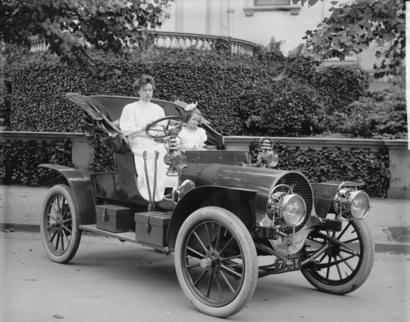
\includegraphics[width=\linewidth]{sample-franklin}
  \caption{1907 Franklin Model D roadster. Photograph by Harris \&
    Ewing, Inc. [Public domain], via Wikimedia
    Commons. (\url{https://goo.gl/VLCRBB}).}
  \Description{A woman and a girl in white dresses sit in an open car.}
\end{figure}

Your figures should contain a caption which describes the figure to
the reader.

Figure captions are placed {\itshape below} the figure.

Every figure should also have a figure description unless it is purely
decorative. These descriptions convey what’s in the image to someone
who cannot see it. They are also used by search engine crawlers for
indexing images, and when images cannot be loaded.

A figure description must be unformatted plain text less than 2000
characters long (including spaces).  {\bfseries Figure descriptions
  should not repeat the figure caption – their purpose is to capture
  important information that is not already provided in the caption or
  the main text of the paper.} For figures that convey important and
complex new information, a short text description may not be
adequate. More complex alternative descriptions can be placed in an
appendix and referenced in a short figure description. For example,
provide a data table capturing the information in a bar chart, or a
structured list representing a graph.  For additional information
regarding how best to write figure descriptions and why doing this is
so important, please see
\url{https://www.acm.org/publications/taps/describing-figures/}.

\subsection{The ``Teaser Figure''}

A ``teaser figure'' is an image, or set of images in one figure, that
are placed after all author and affiliation information, and before
the body of the article, spanning the page. If you wish to have such a
figure in your article, place the command immediately before the
\verb|\maketitle| command:
\begin{verbatim}
  \begin{teaserfigure}
    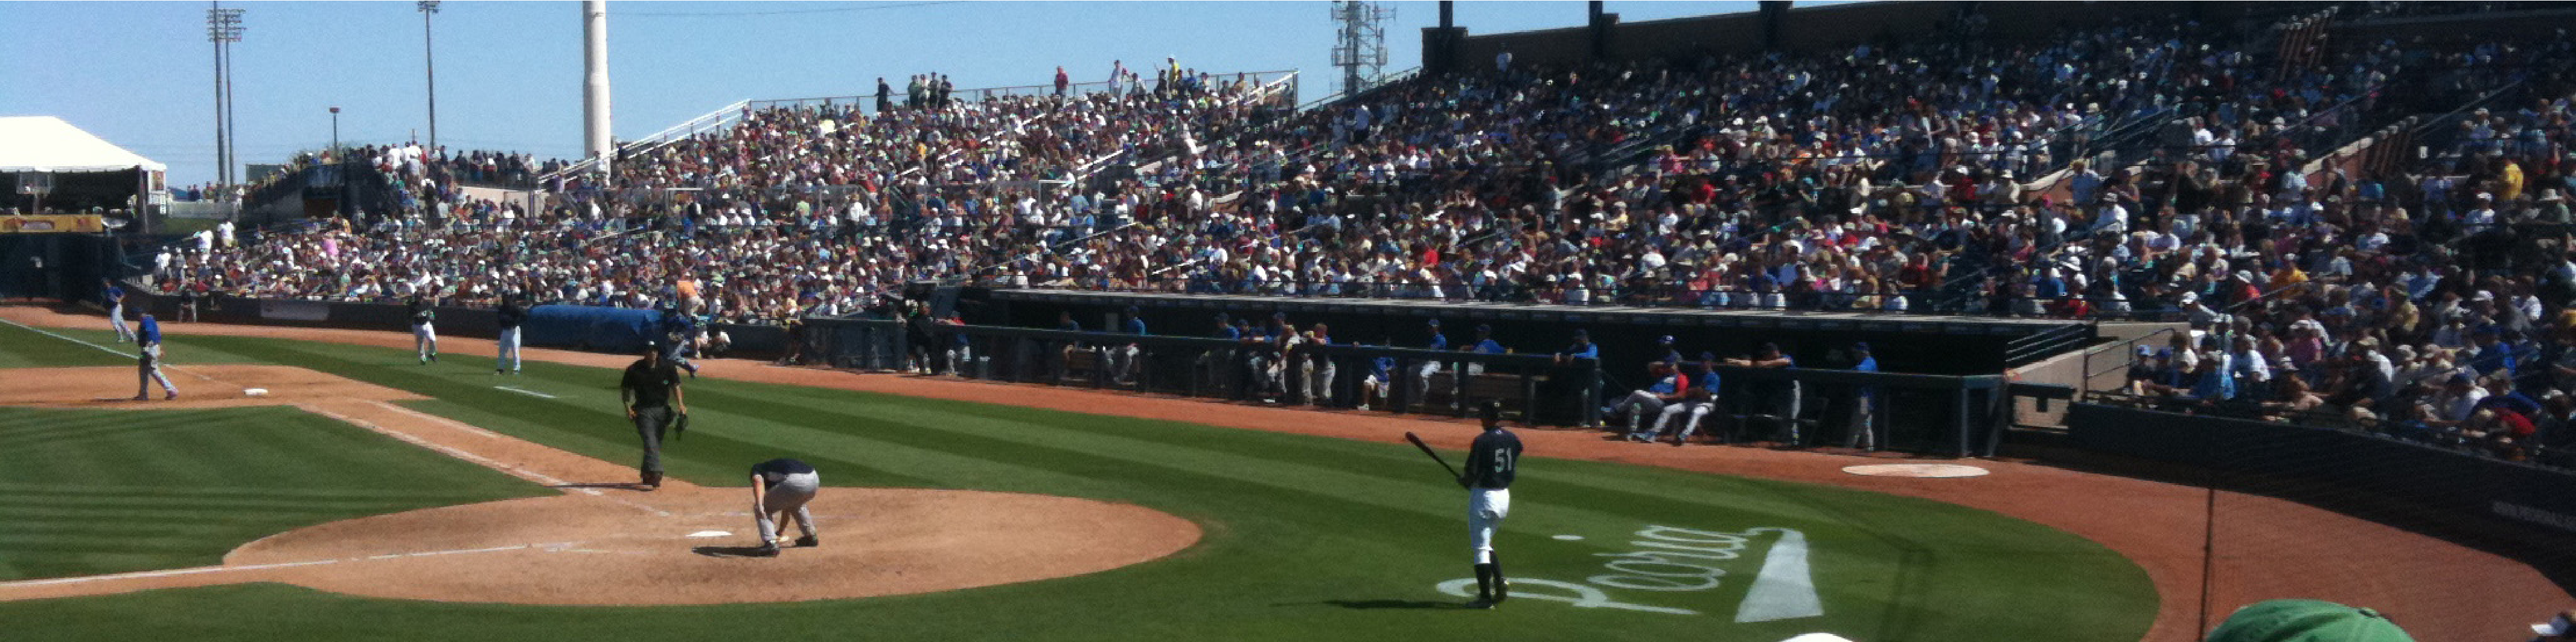
\includegraphics[width=\textwidth]{sampleteaser}
    \caption{figure caption}
    \Description{figure description}
  \end{teaserfigure}
\end{verbatim}

\section{Citations and Bibliographies}

The use of \BibTeX\ for the preparation and formatting of one's
references is strongly recommended. Authors' names should be complete
--- use full first names (``Donald E. Knuth'') not initials
(``D. E. Knuth'') --- and the salient identifying features of a
reference should be included: title, year, volume, number, pages,
article DOI, etc.

The bibliography is included in your source document with these two
commands, placed just before the \verb|\end{document}| command:
\begin{verbatim}
  \bibliographystyle{ACM-Reference-Format}
  \bibliography{bibfile}
\end{verbatim}
where ``\verb|bibfile|'' is the name, without the ``\verb|.bib|''
suffix, of the \BibTeX\ file.

Citations and references are numbered by default. A small number of
ACM publications have citations and references formatted in the
``author year'' style; for these exceptions, please include this
command in the {\bfseries preamble} (before the command
``\verb|\begin{document}|'') of your \LaTeX\ source:
\begin{verbatim}
  \citestyle{acmauthoryear}
\end{verbatim}

  Some examples.  A paginated journal article \cite{Abril07}, an
  enumerated journal article \cite{Cohen07}, a reference to an entire
  issue \cite{JCohen96}, a monograph (whole book) \cite{Kosiur01}, a
  monograph/whole book in a series (see 2a in spec. document)
  \cite{Harel79}, a divisible-book such as an anthology or compilation
  \cite{Editor00} followed by the same example, however we only output
  the series if the volume number is given \cite{Editor00a} (so
  Editor00a's series should NOT be present since it has no vol. no.),
  a chapter in a divisible book \cite{Spector90}, a chapter in a
  divisible book in a series \cite{Douglass98}, a multi-volume work as
  book \cite{Knuth97}, a couple of articles in a proceedings (of a
  conference, symposium, workshop for example) (paginated proceedings
  article) \cite{Andler79, Hagerup1993}, a proceedings article with
  all possible elements \cite{Smith10}, an example of an enumerated
  proceedings article \cite{VanGundy07}, an informally published work
  \cite{Harel78}, a couple of preprints \cite{Bornmann2019,
    AnzarootPBM14}, a doctoral dissertation \cite{Clarkson85}, a
  master's thesis: \cite{anisi03}, an online document / world wide web
  resource \cite{Thornburg01, Ablamowicz07, Poker06}, a video game
  (Case 1) \cite{Obama08} and (Case 2) \cite{Novak03} and \cite{Lee05}
  and (Case 3) a patent \cite{JoeScientist001}, work accepted for
  publication \cite{rous08}, 'YYYYb'-test for prolific author
  \cite{SaeediMEJ10} and \cite{SaeediJETC10}. Other cites might
  contain 'duplicate' DOI and URLs (some SIAM articles)
  \cite{Kirschmer:2010:AEI:1958016.1958018}. Boris / Barbara Beeton:
  multi-volume works as books \cite{MR781536} and \cite{MR781537}. A
  couple of citations with DOIs:
  \cite{2004:ITE:1009386.1010128,Kirschmer:2010:AEI:1958016.1958018}. Online
  citations: \cite{TUGInstmem, Thornburg01, CTANacmart}. Artifacts:
  \cite{R} and \cite{UMassCitations}.

\section{Acknowledgments}

Identification of funding sources and other support, and thanks to
individuals and groups that assisted in the research and the
preparation of the work should be included in an acknowledgment
section, which is placed just before the reference section in your
document.

This section has a special environment:
\begin{verbatim}
  \begin{acks}
  ...
  \end{acks}
\end{verbatim}
so that the information contained therein can be more easily collected
during the article metadata extraction phase, and to ensure
consistency in the spelling of the section heading.

Authors should not prepare this section as a numbered or unnumbered {\verb|\section|}; please use the ``{\verb|acks|}'' environment.

\section{Appendices}

If your work needs an appendix, add it before the
``\verb|\end{document}|'' command at the conclusion of your source
document.

Start the appendix with the ``\verb|appendix|'' command:
\begin{verbatim}
  \appendix
\end{verbatim}
and note that in the appendix, sections are lettered, not
numbered. This document has two appendices, demonstrating the section
and subsection identification method.

\section{SIGCHI Extended Abstracts}

The ``\verb|sigchi-a|'' template style (available only in \LaTeX\ and
not in Word) produces a landscape-orientation formatted article, with
a wide left margin. Three environments are available for use with the
``\verb|sigchi-a|'' template style, and produce formatted output in
the margin:
\begin{itemize}
\item {\verb|sidebar|}:  Place formatted text in the margin.
\item {\verb|marginfigure|}: Place a figure in the margin.
\item {\verb|margintable|}: Place a table in the margin.
\end{itemize}

%%
%% The acknowledgments section is defined using the "acks" environment
%% (and NOT an unnumbered section). This ensures the proper
%% identification of the section in the article metadata, and the
%% consistent spelling of the heading.
\begin{acks}
To Robert, for the bagels and explaining CMYK and color spaces.
\end{acks}

%%
%% The next two lines define the bibliography style to be used, and
%% the bibliography file.
\bibliographystyle{ACM-Reference-Format}
\bibliography{sample-base}

\end{document}
\endinput
%%
%% End of file `sample-sigconf.tex'.
